\documentclass[aspectratio=169,usenames,dvipsnames]{beamer}
\usetheme{metropolis}
%\usecolortheme[snowy,cautious]{owl}
\usecolortheme[snowy]{owl}
\metroset{block=fill}

% For regular math font
\usefonttheme[onlymath]{serif}

\usepackage{appendixnumberbeamer}
\usepackage{booktabs}
\usepackage{fancyvrb}
\usepackage{makecell}
\usepackage{xcolor}
%\usepackage{soul}
\usepackage[normalem]{ulem}
\usepackage{hyperref}
\hypersetup{colorlinks,allcolors=.,urlcolor=blue}
\usepackage{graphicx}
\usepackage{siunitx}
\usepackage[siunitx,europeanresistors,nooldvoltagedirection]{circuitikz}
\usepackage{amsmath}
\usepackage{amssymb}
\usepackage{color}
\usepackage{listings}

% allowframebreaks numbering in the title
\newcounter{cont}
\makeatletter
\setbeamertemplate{frametitle continuation}{%
    \setcounter{cont}{\beamer@endpageofframe}%
    \addtocounter{cont}{1}%
    \addtocounter{cont}{-\beamer@startpageofframe}%
    (\insertcontinuationcount/\arabic{cont})%
}
\makeatother

% Fix dashs/hyphens in listings
\makeatletter
\lst@CCPutMacro\lst@ProcessOther {"2D}{\lst@ttfamily{-{}}{-{}}}
\@empty\z@\@empty
\makeatother

\newfontfamily\Bera{Bitstream Vera Sans Mono}[Scale=1]
\newfontfamily\TgCursor{TeX Gyre Cursor}[Scale=1]
\newfontfamily\Dejavu{DejaVu Sans Mono}[Scale=1]
%\newfontfamily\Consolas{Consolas}[Scale=0.85]
\newfontfamily\Consolas{Consolas}[Scale=1]

% For tikz
\colorlet{darkgreen}{OliveGreen}
\colorlet{darkred}{BrickRed}
% Not used
\definecolor{mygreen}{rgb}{0,0.6,0}
\definecolor{mygray}{rgb}{0.5,0.5,0.5}
\definecolor{mymauve}{rgb}{0.58,0,0.82}
\definecolor{myblue}{rgb}{0,0,1}
% For C
\definecolor{comment}{RGB}{0,128,0} % dark green
\definecolor{string}{RGB}{255,0,0}  % red
\definecolor{keyword}{RGB}{0,0,255} % blue

% Schematic elements colors
\tikzset{
  R/.append style={color=darkred, /tikz/text=black},
  battery1/.append style={color=darkred, /tikz/text=black},
  leDo/.append style={color=darkred, /tikz/text=black},
  short/.append style={color=darkgreen, /tikz/text=black},
  nos/.append style={color=darkred, /tikz/text=black},
  every vcc node/.style={color=darkred, /tikz/text=black},
  every ground node/.style={color=darkred, /tikz/text=black},
  %%% Pin element definition (crossed-out box)
  box/.style={
    rectangle, minimum size=0.5 cm, very thick, draw=black, color=darkred
  },
  pin/.style={
    box,
    append after command={
      [every edge/.append style={
        very thick,
        darkred,
        shorten >=\pgflinewidth,
        shorten <=\pgflinewidth,
      }]
      (\tikzlastnode.north west) edge (\tikzlastnode.south east)
      (\tikzlastnode.north east) edge (\tikzlastnode.south west)
    }
  }
}

\lstdefinestyle{global} {
%  basicstyle=\fontfamily{cmvtt}\selectfont
%  basicstyle=\tiny\ttfamily,
%  basicstyle=\tiny\Dejavu,
  basicstyle=\tiny\Consolas,
  backgroundcolor=\color{white},
  commentstyle=\itshape\color{comment},
  stringstyle=\color{string},
  keywordstyle=\bfseries\color{keyword},
  directivestyle=\bfseries\color{teal},
  %identifierstyle=\bfseries,
  numbers=left,
  numberstyle=\tiny,
  numbersep=5pt,
  frame=lines,
  breaklines=true,
  prebreak=\raisebox{0ex}[0ex][0ex]{\ensuremath{\hookleftarrow}},
  showstringspaces=false,
  upquote=true,
  tabsize=8,
  escapeinside=\`\`,
}

\lstdefinestyle{c} {
  escapeinside=\`\`,
  morekeywords={bool,u8,u16,u32,s8,s16,s32,size_t,ssize_t,inline},
  deletedirectives={line}, % see "kpsewhich lstlang1.sty" file
}

\lstdefinestyle{make} {
  language=make,
  morekeywords={if,ifneq,else,elseif,endif},
}

\lstset {
  language=C,
  style=global,
}


\title{Kernel Course: Lecture 19}
\subtitle{Hardware Tools in Embedded Kernel Development}
\author{Sam Protsenko \texorpdfstring{\\ <joe.skb7@gmail.com>}{}}
\date{\vspace*{5mm}\today}
% \institute{Dark Engineering Initiative}

\begin{document}

% Must be done inside of document, otherwise wrong math fonts will be used
\sisetup {
  math-rm = \mathrm,
  math-micro = \char"00B5, % "micro" sign Unicode, keep this file ASCII
  inter-unit-product = \ensuremath{{}\cdot{}},
  per-mode = fraction,
%  fraction-function = \tfrac,
%  unit-color = purple
}

\maketitle

\begin{frame}{Agenda}
  \setbeamertemplate{section in toc}[sections numbered]
  \tableofcontents[hideallsubsections]
\end{frame}

% ------------------------------------------------------------------------------

\begin{frame}
  \frametitle{Hardware Tools Overview}
  Where it can be useful?
  \begin{itemize}
    \item Debugging hardware issues (obviously)
    \item Board bringup (measuring clocks, voltages, etc)
    \item Fixing adapter drivers
    \item Performance optimizations
    \item Power management optimizations
    \item Investigating low-level components
    \item Debugging subtle problems
  \end{itemize}
\end{frame}

\section{Multimeter}

\begin{frame}
  \frametitle{Multimeter Overview}
  Masures constant electrical values:
  \begin{itemize}
    \item Voltage:
      \begin{itemize}
        \item $ R_V = \infty $
        \item Can be used for power issues diagnostics
        \item Helpful during board bring-up
      \end{itemize}
    \item Current:
      \begin{itemize}
        \item $ R_A = 0 $
        \item \alert{Don't measure the current in power outlets!}
        \item Useful for power management improvements
        \item Sometimes ``10A'' input jack must be used
      \end{itemize}
    \item Resistance:
      \begin{itemize}
        \item Resistors must be unsoldered before measurement
        \item Use beeper mode to check a loop
      \end{itemize}
  \end{itemize}
\end{frame}

\begin{frame}[standout]
  \begin{figure}
    \centering
    \includegraphics[scale=0.8]{images/multimeter.png}
  \end{figure}
  Multimeter Demo: Suspend/Resume Current
\end{frame}

\begin{frame}
  \frametitle{Current Measurement}
  \vspace*{-2mm}
  \begin{columns}
  \column{0.5\textwidth}
    \begin{figure}
      \centering
      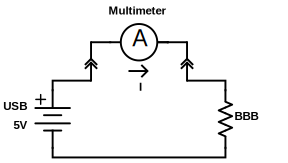
\includegraphics[scale=0.8]{images/ammeter.pdf}
      \caption{Ammeter Connection}
    \end{figure}
  \column{0.5\textwidth}
    \begin{figure}
      \centering
      \includegraphics[scale=0.07]{images/current-cable.jpg}
      \caption{Measurement Cable}
    \end{figure}
  \end{columns}

  Power can be calculated:
  \[ P = V \cdot I \]
\end{frame}

\begin{frame}
  \frametitle{Current Measurement Setup}
  \begin{figure}
    \centering
    \includegraphics[scale=0.07]{images/multimeter-setup.png}
    \caption{Setup for BBB suspend/resume current measurement}
  \end{figure}
  \vspace*{-10mm}
\end{frame}

\begin{frame}
  \frametitle{Measuring BBB suspend/resume current (page 1/3)}
  \begin{figure}
    \centering
    \includegraphics[scale=0.28]{images/multimeter-demo-1.jpg}
    \caption{Current draw: before suspend ($ I = \SI{310}{\mA} $)}
  \end{figure}
  \vspace*{-5mm}
\end{frame}

\begin{frame}
  \frametitle{Measuring BBB suspend/resume current (page 2/3)}
  \begin{figure}
    \centering
    \includegraphics[scale=0.28]{images/multimeter-demo-2.jpg}
    \caption{Current draw: during suspend ($ I = \SI{20}{\mA} $)}
  \end{figure}
  \vspace*{-5mm}
\end{frame}

\begin{frame}
  \frametitle{Measuring BBB suspend/resume current (page 3/3)}
  \begin{figure}
    \centering
    \includegraphics[scale=0.28]{images/multimeter-demo-3.jpg}
    \caption{Current draw: after resume ($ I = \SI{310}{\mA} $)}
  \end{figure}
  \vspace*{-5mm}
\end{frame}

\section{Scope}

\begin{frame}
  \frametitle{Scope Overview}
  \begin{itemize}
    \item Software vs hardware
    \item Parameters: frequency, data rate; + probes (capacity)
    \item Trigger feature
    \item Divisors (/1, /10)
    \item 2 channels (common ground!)
    \item Scale: time, voltage
    \item ``Auto'' button
    \item Measure mode
  \end{itemize}
  \textbf{Useful}:
  \begin{itemize}
    \item To debug fast-changing stuff (can't be done in software)
    \item To see what is actually happening on the line
  \end{itemize}
  \vspace*{-5mm}
\end{frame}

\begin{frame}[standout]
  \frametitle{Demo 1}
  Scope Demo \#1: Measuring Delay
\end{frame}

\begin{frame}
  \frametitle{Button and LED Device}
  \vspace*{-3mm}
  \begin{figure}
    \centering
    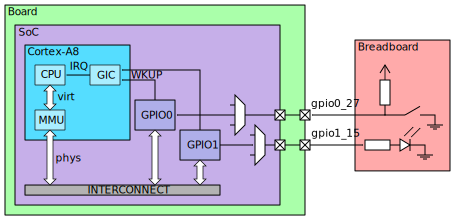
\includegraphics[scale=0.22]{images/architecture2.pdf}
    \caption{Button and LED Device: Functional Block Diagram}
  \end{figure}

  \begin{itemize}
    \item There is a delay between button press and LED toggle events
          (\texttt{hw1.c})
  \end{itemize}
  \vspace*{-2mm}
\end{frame}

\begin{frame}
  \frametitle{Scope Setup}
  \begin{figure}
    \centering
    \includegraphics[scale=0.25]{images/scope-setup.png}
    \caption{Setup for button/LED delay measurement}
  \end{figure}
\end{frame}

\begin{frame}
  \frametitle{Scope Settings}
  \begin{columns}
    \column{0.5\textwidth}
    Channel settings:
    \begin{itemize}
      \item CH1 (blue): Button line
      \item CH2 (yellow): LED line
      \item Coupling: DC
      \item Probe: 10X
      \item Voltage scale: \SI{1}{\volt / div}
      \item Time scale: \SI{1}{\ms / div}
    \end{itemize}

    \column{0.5\textwidth}
    Trigger menu:
    \begin{itemize}
      \item Type: Edge; Slope: Rise,Fall
      \item Source: CH2 (LED line)
      \item Mode: Normal
      \item Coupling: DC
      \item Trigger level: \SI{1}{\volt} (\SI{0}{\volt} ... \SI{3.3}{\volt})
    \end{itemize}
  \end{columns}
\end{frame}

\begin{frame}
  \frametitle{Measuring Delay (page 1/2)}
  \begin{figure}
    \centering
    \includegraphics[scale=0.75]{images/scope-trace-delay1.png}
    \caption{Scope screenshot: LED off \textrightarrow{} on}
  \end{figure}
\end{frame}

\begin{frame}
  \frametitle{Measuring Delay (page 2/2)}
  \begin{figure}
    \centering
    \includegraphics[scale=0.75]{images/scope-trace-delay2.png}
    \caption{Scope screenshot: LED on \textrightarrow{} off}
  \end{figure}
\end{frame}

\begin{frame}[standout]
  \frametitle{Demo 2}
  Scope Demo \#2: Investigating Kernel Sleeps
\end{frame}

\begin{frame}[containsverbatim,allowframebreaks=1]
  \frametitle{Square Wave Module}
  \lstinputlisting[caption=sqw.c, style=c]{materials/sqw/sqw.c}
\end{frame}

\begin{frame}[containsverbatim,allowframebreaks=1]
  \frametitle{Load CPU script}
  \lstinputlisting[caption=\detokenize{load_cpu.sh}, language=bash]
    {materials/sqw/load_cpu.sh}
\end{frame}

\begin{frame}
  \frametitle{Stable Scope Display}
  To make periodic signal ``stand still'', trigger must be configured:
  \begin{itemize}
    \item Type: Edge
    \item Source: CH2
    \item Slope: Rise
    \item Mode: Auto
    \item Coupling: DC
    \item Trigger level: put it in the wave center
  \end{itemize}

  Or just use ``Auto'' button to configure that for you.
\end{frame}

\begin{frame}
  \frametitle{Checking Square Wave (page 1/2)}
  \begin{figure}
    \centering
    \includegraphics[scale=0.75]{images/scope-trace-sqw1.png}
    \caption{Scope screenshot: CPU load 0\%}
  \end{figure}
\end{frame}

\begin{frame}
  \frametitle{Checking Square Wave (page 2/2)}
  \begin{figure}
    \centering
    \includegraphics[scale=0.75]{images/scope-trace-sqw2.png}
    \caption{Scope screenshot: CPU load 100\%}
  \end{figure}
\end{frame}

\begin{frame}[standout]
  \frametitle{Demo 3}
  Scope Demo \#3: Investigating I2C Transmission
\end{frame}

\begin{frame}
  \frametitle{Probes}
  \begin{columns}
    \column{0.6\textwidth}
      \begin{itemize}
        \item Use ``10X'' mode for regular operation:
          \begin{itemize}
            \item $ C_{in} = \SI{20}{\pF} \Rightarrow T = R_{PU} \cdot C_{in} = \SI{50}{\kohm} \cdot \SI{20}{\pF} = \SI{1}{\us} $
          \end{itemize}
        \item Use ``1X'' mode for low voltage signals:
          \begin{itemize}
            \item $ C_{in} = \SI{100}{\pF} \Rightarrow T = R_{PU} \cdot C_{in} = \SI{50}{\kohm} \cdot \SI{100}{\pF} = \SI{5}{\us} $
          \end{itemize}
      \end{itemize}
  \vspace*{5mm}
  \[ T_{SDC} = \frac{1}{\SI{100}{\kHz}} = \SI{10}{\us} \]
    \column{0.4\textwidth}
      \begin{figure}
        \centering
          \hspace*{-5mm}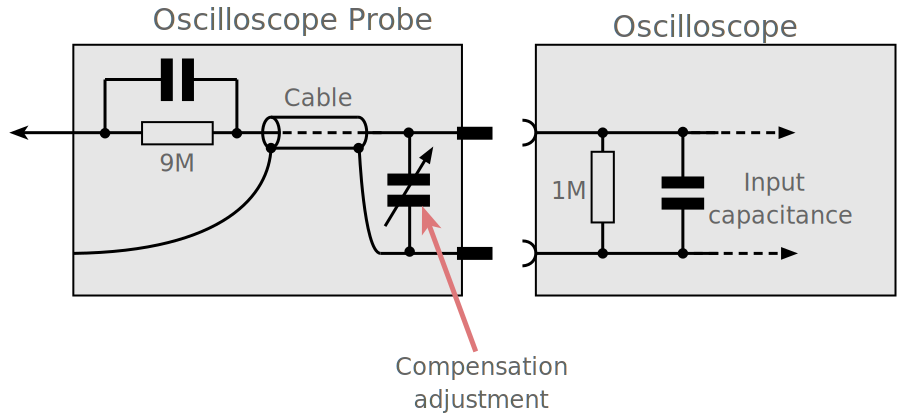
\includegraphics[scale=0.27]{images/scope-probe-x10-circuit.pdf}\hspace*{-4mm}
        \caption{Oscilloscope probe (X10) circuit}
      \end{figure}
  \end{columns}
\end{frame}

\begin{frame}
  \frametitle{Checking I2C Transmission (page 1/2)}
  \begin{figure}
    \centering
    \includegraphics[scale=0.75]{images/scope-trace-i2c-x1.png}
    \caption{Scope screenshot: I2C Transmission using X1 probe}
  \end{figure}
\end{frame}

\begin{frame}
  \frametitle{Checking I2C Transmission (page 2/2)}
  \begin{figure}
    \centering
    \includegraphics[scale=0.75]{images/scope-trace-i2c-x10.png}
    \caption{Scope screenshot: I2C Transmission using X10 probe}
  \end{figure}
\end{frame}

\section{Logic Analyzer}

\begin{frame}
  \frametitle{Logic Analyzer Overview}
  \begin{columns}
    \column{0.5\textwidth}
    \begin{itemize}
      \item Catches digital levels
      \item Stores collected data to internal (hardware) buffer
      \item App can parse protocols (I2C, UART)
      \item Parameters: max data rate (freq), ports count, protocols support
      \item Some specialized LAs exist (e.g. USB)
      \item \textbf{Useful}:
        \begin{itemize}
          \item For problem isolation / root-causing
          \item For reverse engineering (``sniffing'')
        \end{itemize}
    \end{itemize}
    \column{0.5\textwidth}
    \begin{figure}
      \centering
      \hspace*{-2mm}\includegraphics[scale=0.17]{images/saleae-la.jpg}
      \caption{Saleae 16 Logic Analyzer}
    \end{figure}
  \end{columns}
\end{frame}

\begin{frame}[standout]
  \frametitle{Demo 1}
  LA Demo \#1: I2C (SDA, SCL)
\end{frame}

\begin{frame}
  \frametitle{I2C data exchange with RTC (page 1/3)}
  \begin{figure}
    \centering
    \includegraphics[scale=0.38]{images/la-i2c-window.png}
    \caption{I2C data exchange with DS1307 sniffed by Logic Analyzer}
  \end{figure}
  \vspace*{-10mm}
\end{frame}

\begin{frame}[containsverbatim]
  \frametitle{I2C data exchange with RTC (page 2/3)}
  \begin{figure}
    \centering
    \includegraphics[scale=0.55]{images/la-i2c-read.png}
    \caption{I2C read from 0x01 register}
  \end{figure}
  \begin{lstlisting}[numbers=none]
[15347.357045] ### my_rtc probe(): enter
[15347.362433] ### read data = 0x15
  \end{lstlisting}
  \vspace*{-5mm}
\end{frame}

\begin{frame}[containsverbatim]
  \frametitle{I2C data exchange with RTC (page 3/3)}
  \vspace*{-1mm}
  \begin{figure}
    \centering
    \includegraphics[scale=0.5]{images/la-i2c-read-bulk.png}
    \caption{I2C bulk read (starting from 0x00 register)}
  \end{figure}
  \begin{lstlisting}[numbers=none]
[15347.368436] ds1307x 2-0068: reg 0x0  = 0xd4
[15347.372824] ds1307x 2-0068: reg 0x1  = 0x15
[15347.377113] ds1307x 2-0068: reg 0x2  = 0x4
[15347.381395] ds1307x 2-0068: reg 0x3  = 0x1
[15347.385593] ds1307x 2-0068: reg 0x4  = 0x1
[15347.389808] ds1307x 2-0068: reg 0x5  = 0x1
[15347.394005] ds1307x 2-0068: reg 0x6  = 0x0
  \end{lstlisting}
  \vspace*{-7mm}
\end{frame}

\begin{frame}[standout]
  \frametitle{Demo 2}
  LA Demo \#2: UART (Tx, Rx)
\end{frame}

\begin{frame}
  \frametitle{LA UART Setup}
  \begin{figure}
    \centering
    \includegraphics[scale=0.087]{images/la-uart-setup.png}
    \vspace*{-1mm}
    \caption{Setup for tracing UART with Logic Analyzer}
  \end{figure}
  \vspace*{-7mm}
\end{frame}

\begin{frame}
  \frametitle{UART data exchange with serial console (page 1/3)}
  \begin{figure}
    \centering
    \includegraphics[scale=0.32]{images/la-uart-window.png}
    \vspace*{-1mm}
    \caption{UART data exchange with FTDI sniffed by Logic Analyzer}
  \end{figure}
  \vspace*{-11mm}
\end{frame}

\begin{frame}
  \frametitle{UART data exchange with serial console (page 2/3)}
  \begin{figure}
    \centering
    \includegraphics[scale=0.55]{images/la-uart-char.png}
    \caption{Type in `\texttt{p}' character and get it back in minicom}
  \end{figure}
\end{frame}

\begin{frame}
  \frametitle{UART data exchange with serial console (page 3/3)}
  \begin{figure}
    \centering
    \hspace*{-8mm}\includegraphics[scale=0.5]{images/la-uart-pwd.png}\hspace*{-8mm}
    \caption{\texttt{pwd} command response}
  \end{figure}
\end{frame}

\begin{frame}[standout]
  Take Five
\end{frame}

\section{JTAG}

\begin{frame}
  \frametitle{JTAG Intro}
  Allows one to debug program running on board just like user-space application
  with GDB:
  \begin{itemize}
    \item Breakpoints
    \item Read/write registers
    \item Stop/run CPU
    \item Read/write memory
    \item Load images
    \item Examine stack
    \item Can debug U-Boot, kernel, user-space apps/libs, even ROM-code...
  \end{itemize}
\end{frame}

\begin{frame}
  \frametitle{JTAG Bus}
  \begin{figure}
    \centering
    \includegraphics[scale=0.45]{images/jtag_chain.pdf}
    \caption{Daisy-chained JTAG}
  \end{figure}
  \begin{itemize}
    \item JTAG is a serial bus (IEEE1149.1 standard)
    \item AM335x implements JTAG (has JTAG pins)
    \item PC doesn't have JTAG controller, so \textbf{JTAG adapter} must be used
  \end{itemize}
\end{frame}

\begin{frame}
  \frametitle{JTAG Adapters}
  \begin{figure}
    \centering
    \includegraphics[scale=0.6]{images/jtag-sw.pdf}
    \caption{Connecting BBB JTAG to PC}
  \end{figure}
  Adapters require some software. Some examples for BBB:
    \begin{itemize}
      \item \textbf{Flyswatter 2} (FT2232H based, MPSSE): OpenOCD
      \item \textbf{XDS100v2}: Proprietary software
    \end{itemize}
\end{frame}

\begin{frame}
  \frametitle{JTAG support in AM335x}
  \begin{figure}
    \centering
    \hspace*{-2mm}\includegraphics[scale=0.33]{images/jtag-bbb-scheme.pdf}\hspace*{-2mm}
    \caption{JTAG connector in BBB}
  \end{figure}
  See TRM for details on debug interface implementation in AM335x.
\end{frame}

\begin{frame}
  \frametitle{Flyswatter2 Overview}
  \begin{columns}
    \column{0.4\textwidth}
      \begin{figure}
        \centering
        \includegraphics[scale=0.3]{images/bbb-connector.jpg}
        \caption{BBB JTAG Connector}
      \end{figure}
    \column{0.6\textwidth}
      \begin{figure}
        \centering
        \includegraphics[scale=0.32]{images/bbb-and-flyswatter.jpg}
        \caption{BBB and Flyswatter2}
      \end{figure}
  \end{columns}
  \vspace*{-5mm}
\end{frame}

\begin{frame}[containsverbatim]
  \frametitle{OpenOCD Overview}
  \begin{figure}
    \centering
    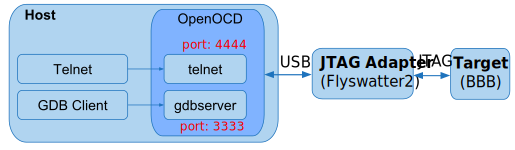
\includegraphics[scale=0.6]{images/openocd.pdf}
    \caption{Debugging BBB with OpenOCD}
  \end{figure}
  \begin{columns}
    \column{0.5\textwidth}
      OpenOCD creates servers for:
      \begin{itemize}
        \item Telnet (port 4444 on localhost)
        \item GDB (port 3333 on localhost)
      \end{itemize}
    \column{0.5\textwidth}
      Once OpenOCD is running, you can run:
      \begin{lstlisting}
        $ telnet localhost 4444
          `or`
        $ arm-eabi-gdb vmlinux
      \end{lstlisting}
  \end{columns}
\end{frame}

\begin{frame}
  \frametitle{Kernel Preparations}
  \begin{itemize}
    \item Enable \texttt{CONFIG\_DEBUG\_INFO} (the same as \texttt{-g})
    \item Disable \texttt{CONFIG\_WATCHDOG} (just in case)
    \item Make sure JTAG clock (DEBUGSS on BBB) is alive in kernel
          (see next slide)
    \item Rebuild, add \texttt{zImage} to rootfs, flash to BBB
  \end{itemize}
\end{frame}

\begin{frame}[containsverbatim]
  \frametitle{Kernel Preparations (cont'd)}
  \texttt{arch/arm/mach-omap2/omap\_hwmod\_33xx\_data.c}:
  \begin{lstlisting}
static struct omap_hwmod am33xx_debugss_hwmod = {
        .name           = "debugss",
        .class          = &am33xx_debugss_hwmod_class,
        .clkdm_name     = "l3_aon_clkdm",
+       .flags          = (HWMOD_INIT_NO_IDLE | HWMOD_INIT_NO_RESET),
        .main_clk       = "trace_clk_div_ck",
        .prcm           = {
  \end{lstlisting}
  Without this patch you'll see \texttt{STICKY BIT} errors (in OpenOCD terminal)
  when kernel starts running.
\end{frame}

\begin{frame}[containsverbatim]
  \frametitle{OpenOCD Preparations}
  Install OpenOCD (my version is 0.10.0):
  \begin{lstlisting}[language=bash]
`\$` sudo apt update
`\$` sudo apt install openocd
  \end{lstlisting}

  \begin{itemize}
    \item Figure out correct OpenOCD interface and target config files:\\
      \begin{itemize}
        \item \texttt{interface/ftdi/flyswatter2.cfg}
        \item \texttt{target/am335x.cfg}
      \end{itemize}
    \item ...but those files from upstream OpenOCD won't work
    \item Use Flyswatter2 config from TinCanTools site (see next page)
%    \item Come up with correct OpenOCD run command (or board configuration)
%    \item Use correct adapter frequency (\SI{1000}{\kilo\hertz} for Flyswatter2)
  \end{itemize}
\end{frame}

\begin{frame}[containsverbatim,allowframebreaks=1]
  \frametitle{OpenOCD Working Script for Flyswatter2}
  \lstinputlisting[language=tcl,caption=ti\_beaglebone\_with\_fs2\_mod.cfg]{materials/ti_beaglebone_with_fs2_mod.cfg}
\end{frame}

\begin{frame}[containsverbatim]
  \frametitle{Run OpenOCD}
  \begin{enumerate}
  \item Connect Flyswatter2 to BBB using adapter kit
  \item Connect Flyswatter2 to PC via USB
  \item Connect BBB to PC via USB (power); \\
        ``TARGET RESET'' LED on Flyswatter is glowing, CPU is in reset state
  \item Run OpenOCD command:
    \begin{lstlisting}[language=bash,numbers=none]
`\$` openocd -f ./ti_beaglebone_with_fs2_mod.cfg -c "init" -c "reset init"
    \end{lstlisting}
  We will use this terminal to track OpenOCD log.
  \end{enumerate}
\end{frame}

\begin{frame}[containsverbatim]
  \frametitle{Correct OpenOCD Command Output}
  \vspace*{-5mm}
  \begin{lstlisting}[numbers=none]
adapter speed: 16000 kHz
Info : auto-selecting first available session transport "jtag". To override use 'transport select <transport>'.
Warn : target name is deprecated use: 'cortex_a'
trst_and_srst separate srst_gates_jtag trst_push_pull srst_open_drain connect_deassert_srst
Info : ftdi: if you experience problems at higher adapter clocks, try the command "ftdi_tdo_sample_edge falling"
Info : clock speed 16000 kHz

`\textbf{Info : JTAG tap: am335x.jrc tap/device found: 0x2b94402f (mfg: 0x017 (Texas Instruments), part: 0xb944, ver: 0x2)}`
Info : JTAG tap: am335x.dap enabled
Info : DAP transaction stalled (WAIT) - slowing down
Info : DAP transaction stalled (WAIT) - slowing down
Info : DAP transaction stalled (WAIT) - slowing down
Error: target->coreid 0 powered down!

`\textbf{Info : JTAG tap: am335x.jrc tap/device found: 0x2b94402f (mfg: 0x017 (Texas Instruments), part: 0xb944, ver: 0x2)}`
Info : JTAG tap: am335x.dap enabled
Info : DAP transaction stalled (WAIT) - slowing down
Info : DAP transaction stalled (WAIT) - slowing down
Info : DAP transaction stalled (WAIT) - slowing down
Info : am335x.cpu: hardware has 6 breakpoints, 2 watchpoints
  \end{lstlisting}
  \vspace*{-5mm}
\end{frame}

\begin{frame}[containsverbatim]
  \frametitle{OpenOCD over GDB (page 1)}
  Let's start debug session in GDB:
  \begin{lstlisting}[numbers=none]
    `\$` arm-eabi-gdb vmlinux

    (gdb) target remote localhost:3333
    (gdb) monitor cortex_a dacrfixup on
    (gdb) continue
  \end{lstlisting}
  What we did here:
  \begin{enumerate}
    \item Connect to OpenOCD's GDB server, using Linux kernel symbols
    \item Using OpenOCD \texttt{cortex\_a} command, do a workaround for software
          breakpoints (Linux kernel maps \texttt{.text} read-only, and the
          debugger cannot write a breakpoint due to that)
    \item Continue CPU execution (as it was in reset state initially);\\
          we use GDB commands for debugging (not \texttt{monitor resume}, etc)
  \end{enumerate}
\end{frame}

\begin{frame}[containsverbatim]
  \frametitle{OpenOCD over GDB (page 2)}
  \vspace*{-5mm}
  Set a breakpoint and trigger it:
  \begin{lstlisting}[numbers=none]
    ^C
    (gdb) break do_sys_open
    (gdb) continue

    / # cat /proc/cmdline
  \end{lstlisting}
  \begin{enumerate}
    \item Stop CPU execution by pressing \texttt{Ctrl-C}
    \item Set breakpoint for \texttt{do\_sys\_open()} kernel function (it's a
          handler for \texttt{open()} syscall. Another interesting functions
          would be \texttt{load\_module()}, \texttt{start\_kernel()}, etc
    \item Continue CPU execution
    \item Print \texttt{/proc/cmdline} file, so that \texttt{open()} is
          triggered
    \item Now we are in breakpoint, CPU is halted
  \end{enumerate}
  \vspace*{-5mm}
\end{frame}

\begin{frame}[containsverbatim]
  \frametitle{OpenOCD over GDB (page 3)}
  Investigate code in breakpoint:
  \begin{lstlisting}[numbers=none]
    (gdb) monitor cortex_a maskisr on
    (gdb) continue
    (gdb) ...
    (gdb) bt, list, info registers, disas, step, print, ...
    (gdb) monitor cortex_a maskisr off
    (gdb) continue
  \end{lstlisting}
  \begin{enumerate}
    \item Don't process interrupts when stepping (otherwise we won't be
          able to perform \texttt{continue})
    \item Wait for \texttt{open("/proc/cmdline")}
    \item Investigate caught code
    \item Once we are done, enable interrupts processing and continue normal
          execution
  \end{enumerate}
\end{frame}

\begin{frame}[containsverbatim]
  \frametitle{OpenOCD Telnet Commands}
  In Telnet, you can use regular OpenOCD monitor commands:
  \begin{itemize}
    \item help
    \item reset
    \item halt
    \item resume
    \item reg
    \item bp <address> <len> [hw]
    \item step [address]
    \item mdw, mww
  \end{itemize}
  See \textbf{OpenOCD User's Guide} for details.
\end{frame}

\begin{frame}
  \frametitle{Proprietary JTAG: XDS100v2 via CodeComposerStudio}
  \begin{figure}
    \centering
    \includegraphics[scale=0.32]{images/uboot-jtag.png}
  \end{figure}
  \vspace*{-10mm}
\end{frame}

%\begin{frame}
%  \frametitle{XDS100v2 JTAG: Video}
%\includemedia[width=0.95\linewidth,height=0.534\linewidth,activate=pageopen,
%passcontext,
%transparent,
%addresource=materials/kernel-jtag-ccs.avi,
%flashvars={source=materials/kernel-jtag-ccs.avi}
%]{\includegraphics[width=0.6\linewidth]{images/kernel-jtag-ccs.png}}{VPlayer.swf}
%  \vspace*{-10mm}
%\end{frame}

\begin{frame}[standout]
  \frametitle{Demo}
  JTAG Demo \#1: Flyswatter2
\end{frame}

\begin{frame}[standout]
  \frametitle{Demo}
  JTAG Demo \#2: XDS560v2
\end{frame}

\begin{frame}
  \frametitle{JTAG References}
  \begin{itemize}
    \item \url{https://www.tincantools.com/flyswatter2-beaglebone-black-how-to/}
    \item \url{https://e2e.ti.com/support/embedded/linux/f/354/t/363421}
    \item \url{https://www.tincantools.com/beaglebone-black-eclipse-gdb/}
    \item \url{https://devel.rtems.org/wiki/Debugging/OpenOCD/BeagleBoneBlack}
    \item \url{https://elinux.org/Debugging\_The\_Linux\_Kernel\_Using\_Gdb}
    \item \url{https://github.com/n-aizu/freertos-multicore/wiki/Debugging-with-openocd}
    \item \url{http://openocd.org/doc/html/GDB-and-OpenOCD.html}
    \item \url{http://openocd.org/doc/html/General-Commands.html}
    \item \url{https://habr.com/post/206036/}
  \end{itemize}
  \vspace*{-10mm}
\end{frame}

\begin{frame}[standout]
  Thank you!
\end{frame}

\end{document}
